\chapter{Evaluation}

\section{Customer Requirements}

\subsection{General Objectives}

\begin{itemize}
	\item Easy to input new data and change existing data
	\item Automatically able to print new invoices by selecting a name with data straight from the database
	\item Clean and easy to understand database with no redundant data.
	\item Secure data, especially as the database does contain data relating to minors.
\end{itemize}

\subsection{Core Objectives}
\begin{itemize}
	\item Able to input new data
	\item Able to easily print an invoice
\end{itemize}


%include as many subsections as necessary for your objectives
\subsection{Objective Evaluation}

\subsubsection{General Objectives}
\underline{Objective 1: Easy to input new data and change existing data}
This objective was met due to the program's ability to enter data in line edits and its ability to edit data directly in the table. The line edits are labeled with ghost text describing what should go in that field. I could not conceive of a better way to perform either of these functions. Both functions work well with little errors or problems.

\begin{figure}[H]
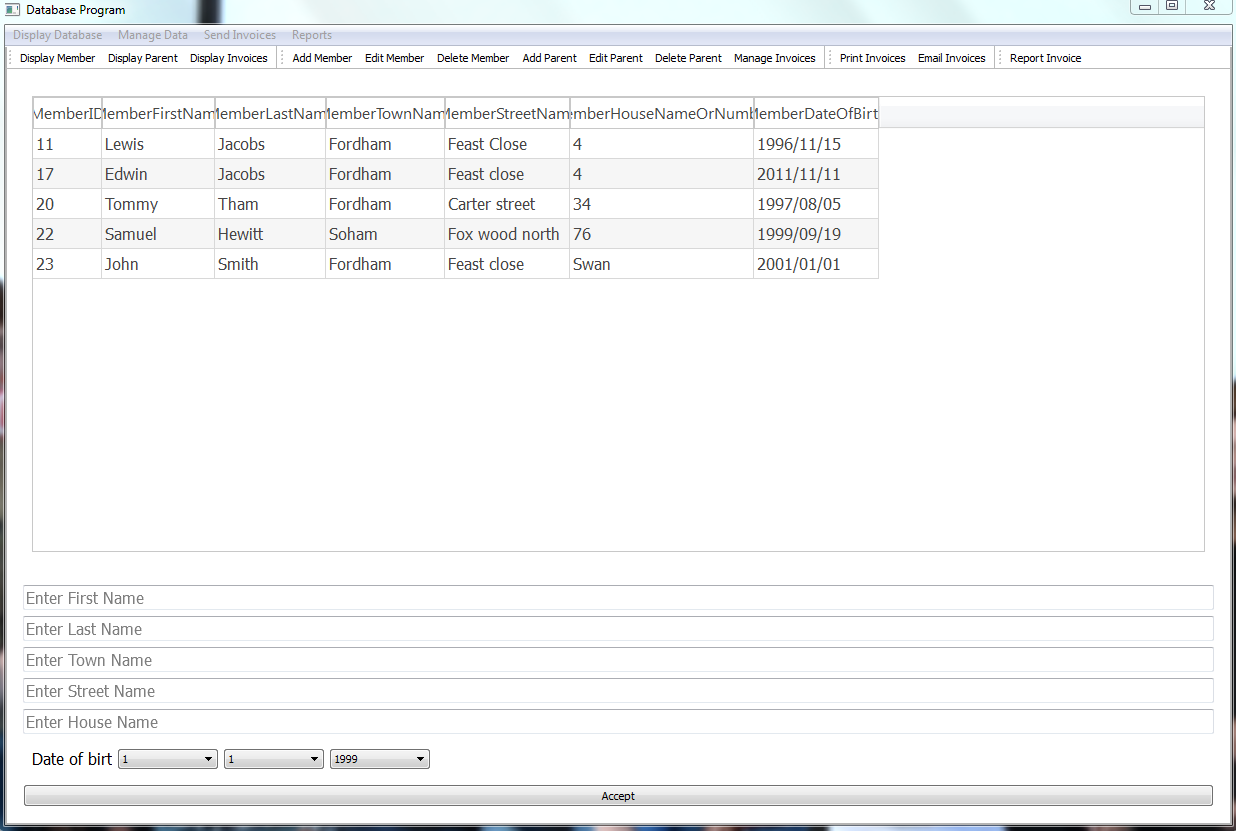
\includegraphics[width=\textwidth]{./Evaluation/Images/AddMember.png}
    \caption{Adding a member} \label{fig:add_member}
\end{figure}
Figure \ref{add_member} shows that the line edits have ghost text in them to show the user where to put which data.

\begin{figure}[H]
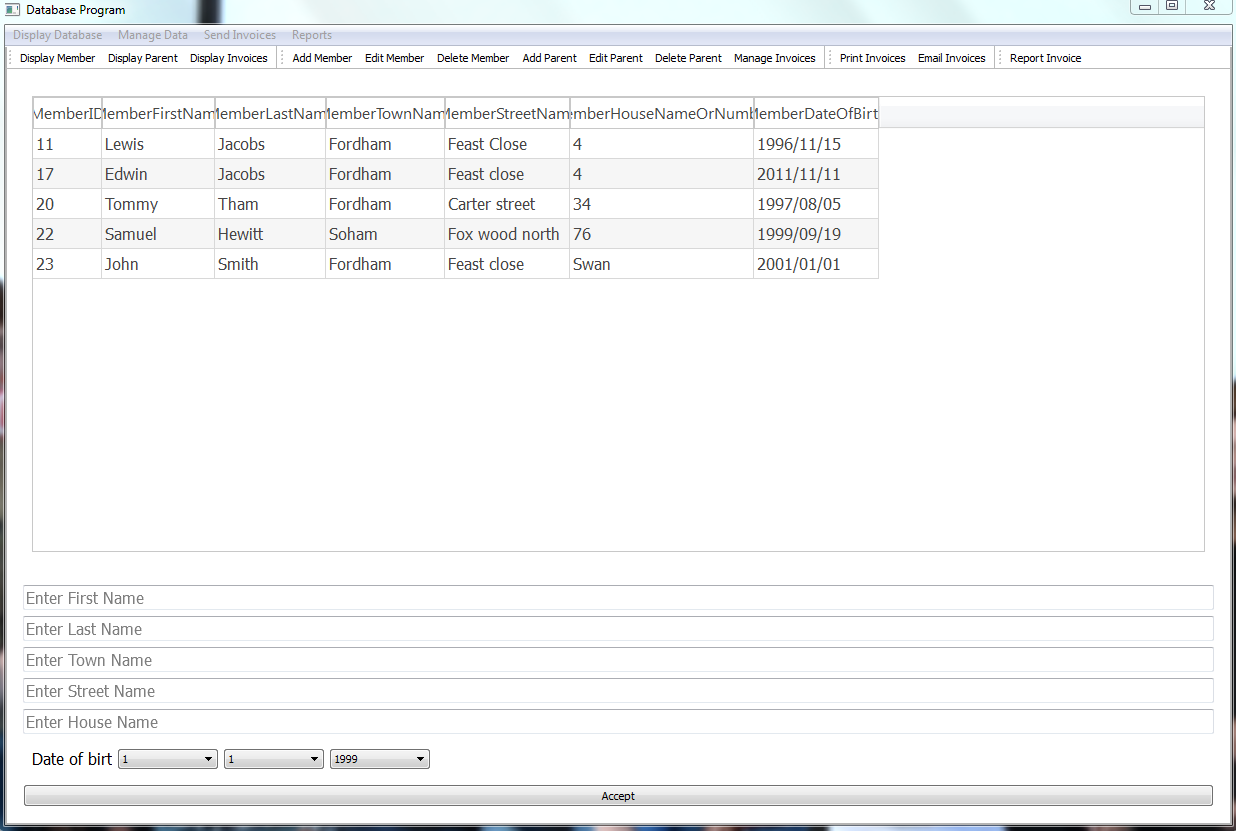
\includegraphics[width=\textwidth]{./Evaluation/Images/AddMember.png}
    \caption{Adding a member} \label{fig:add_member}
\end{figure}

\underline{Objective 2: Automatically able to print new invoices by selecting a name with data straight from the database}
This objective was not met as although the program is able to print a template of the invoice data cannot be selected or a member chosen. I failed to complete this function due to to time restraints.

\underline{Objective 3: Clean and easy to understand database with no redundant data}
This objective was partially met. The database is displayed well however the columns should have been titled with easy to understand names like "First Name" rather than "MemberFirstName". Although data is validated before it is put in the database there is nothing stopping the user inputing the same data twice or inputting wrong data, even if it is valid. Additionally, there is no validation when editing data.

\underline{Objective 4: Secure data, especially as the database does contain data relating to minors}
This objective was partially met. A username and password are required to access the program, both of which are stored in a binary file that cannot be easily read. However, the data can be viewed easily by an external program.

\subsubsection{Specific Objectives}
\underline{Data is input one field at a time via a GUI}


\underline{If the data input is not valid it will ask for only the incorrect field to be re-entered}


\underline{Data can be changed by selecting the record and field wishing to be changed}


\underline{Able to delete a whole record at once}


\section{Effectiveness}

%include as many subsections as necessary for your objectives
\subsection{Objective Evaluation}

\subsubsection{General Objectives}
\underline{Objective 1: Easy to input new data and change existing data}
This objective was met due

\underline{Objective 2: Automatically able to print new invoices by selecting a name with data straight from the database}
This objective was not met

\underline{Objective 3: Clean and easy to understand database with no redundant data}
This objective was partially met

\underline{Objective 4: Secure data, especially as the database does contain data relating to minors}
This objective was partially met


\section{Learnability}
My client is well versed in computers and IT and uses Excel spreadsheets almost every day, so my program does not need a gradual learning curve. However, if my client decides to pass on leadership of scouts then his predecessor will need to know how to use the program, and it is impossible to tell what kind of IT skills they may have, so I have tried to keep my program simple.

The program is laid out similarly to any other database program, with sections easy accessible via buttons at the top of the screen and tables in the database displayed in every screen, so that the program seemed familiar.

As none of the features of my program are particularly complex, learning every function of the program should take only few minutes from someone with even basic computer skills, especially with someone who has used the program before guiding the user.

\section{Usability}

\section{Maintainability}

\section{Suggestions for Improvement}
My program would have been vastly improved if I had had more time to finish the finer features of the program.

More time would also have enabled me to clean up the code, especially with regards to classes and reusing the validation functions.

\underline{Version 2.0}
I believe that if my client will use my program I will continue to work on my program and add to it until I am satisfied with it, which I am currently not. I would firstly fix the bugs identified in my testing section, most of which I know how to easily fix, and ensure that printing and emailing invoices work as they should. I would then format the tables with correct headings and column widths before moving on to adding a warning system that ensures that the user wants to delete that entity when it is double clicked. 

\section{End User Evidence}

\subsection{Questionnaires}

\subsection{Graphs}

\subsection{Written Statements}





